\chapter{Implementation}
  Used language: python\newline
  Why python and not c/c++?
    Rapid prototyping, easier debugging, easier accessible, module separation, no further stress on wlc/aps because runs on admins client pc, networkx library already existant
  \begin{figure}[t]
    \centering
    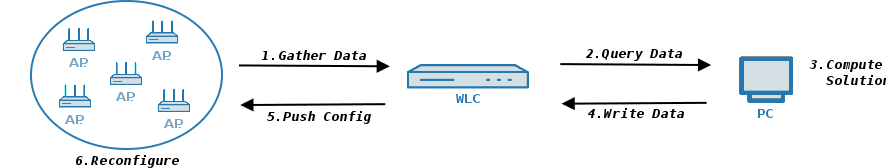
\includegraphics[width=1\columnwidth]{figures/dataflow}
    \label{fig:dataflow}
  \end{figure}
\section{Dependencies}
  \begin{description}
   \item[Which Modules have been included/imported?]
   \item[What is the purpose of those modules in our code?]
   \item[Have we extended the modules?]
   Yes, Python collections -> added additional methods for convencience
  \end{description}
\section{Structure of the code}
  Rather similar structure like algorithm -> split into two sections
  \subsection{Selecting the Network Topology}
    \subsubsection{Minimal Spanning Tree}
    \subsubsection{Adding Redundand Paths}
  \subsection{Coloring the Edges/Modules}
\section{Problems}
  \begin{description}
   \item[Have there been problems with the implementation?]
   Actually no
   \item[What else could count as a problem / What else could fit in here?]
  \end{description}
\section{Run it yourself}
  \begin{description}
   \item[What is needed to run the algorithm on your own machine?]
    Input data is required (aka which access point sees what other acces point with what Signal to Noise Ratio?) \newline
  \end{description}
